\label{sec:experiments}

We evaluate TrianguLang on multi-view semantic segmentation across five benchmarks, comparing against click-based and optimization-based methods.

\subsection{Experimental Setup}

\paragraph{Datasets.}
We evaluate on five multi-view benchmarks:
\begin{itemize}[nosep,leftmargin=*]
    \item \textbf{ScanNet++}~\cite{scannet++}: Indoor scenes with dense semantic annotations. We train on the \texttt{nvs\_sem\_train} split (230 scenes) and evaluate on a separate held-out \texttt{nvs\_sem\_val} split (50 scenes).
    \item \textbf{uCO3D}~\cite{UCo3D}: Object-centric 360$^\circ$ captures across 1,000 categories.
    \item \textbf{LERF-OVS}~\cite{lerf}: 4 tabletop scenes with per-frame language-grounded annotations for open-vocabulary segmentation and localization.
    \item \textbf{NVOS}~\cite{NVOS}: 6 multi-view object selection scenes.
    \item \textbf{SPIn-NeRF}~\cite{spinnerf}: 10 real-world multi-view scenes.
\end{itemize}

% Figure moved to appendix for space
\begin{figure}[h]
\begin{center}
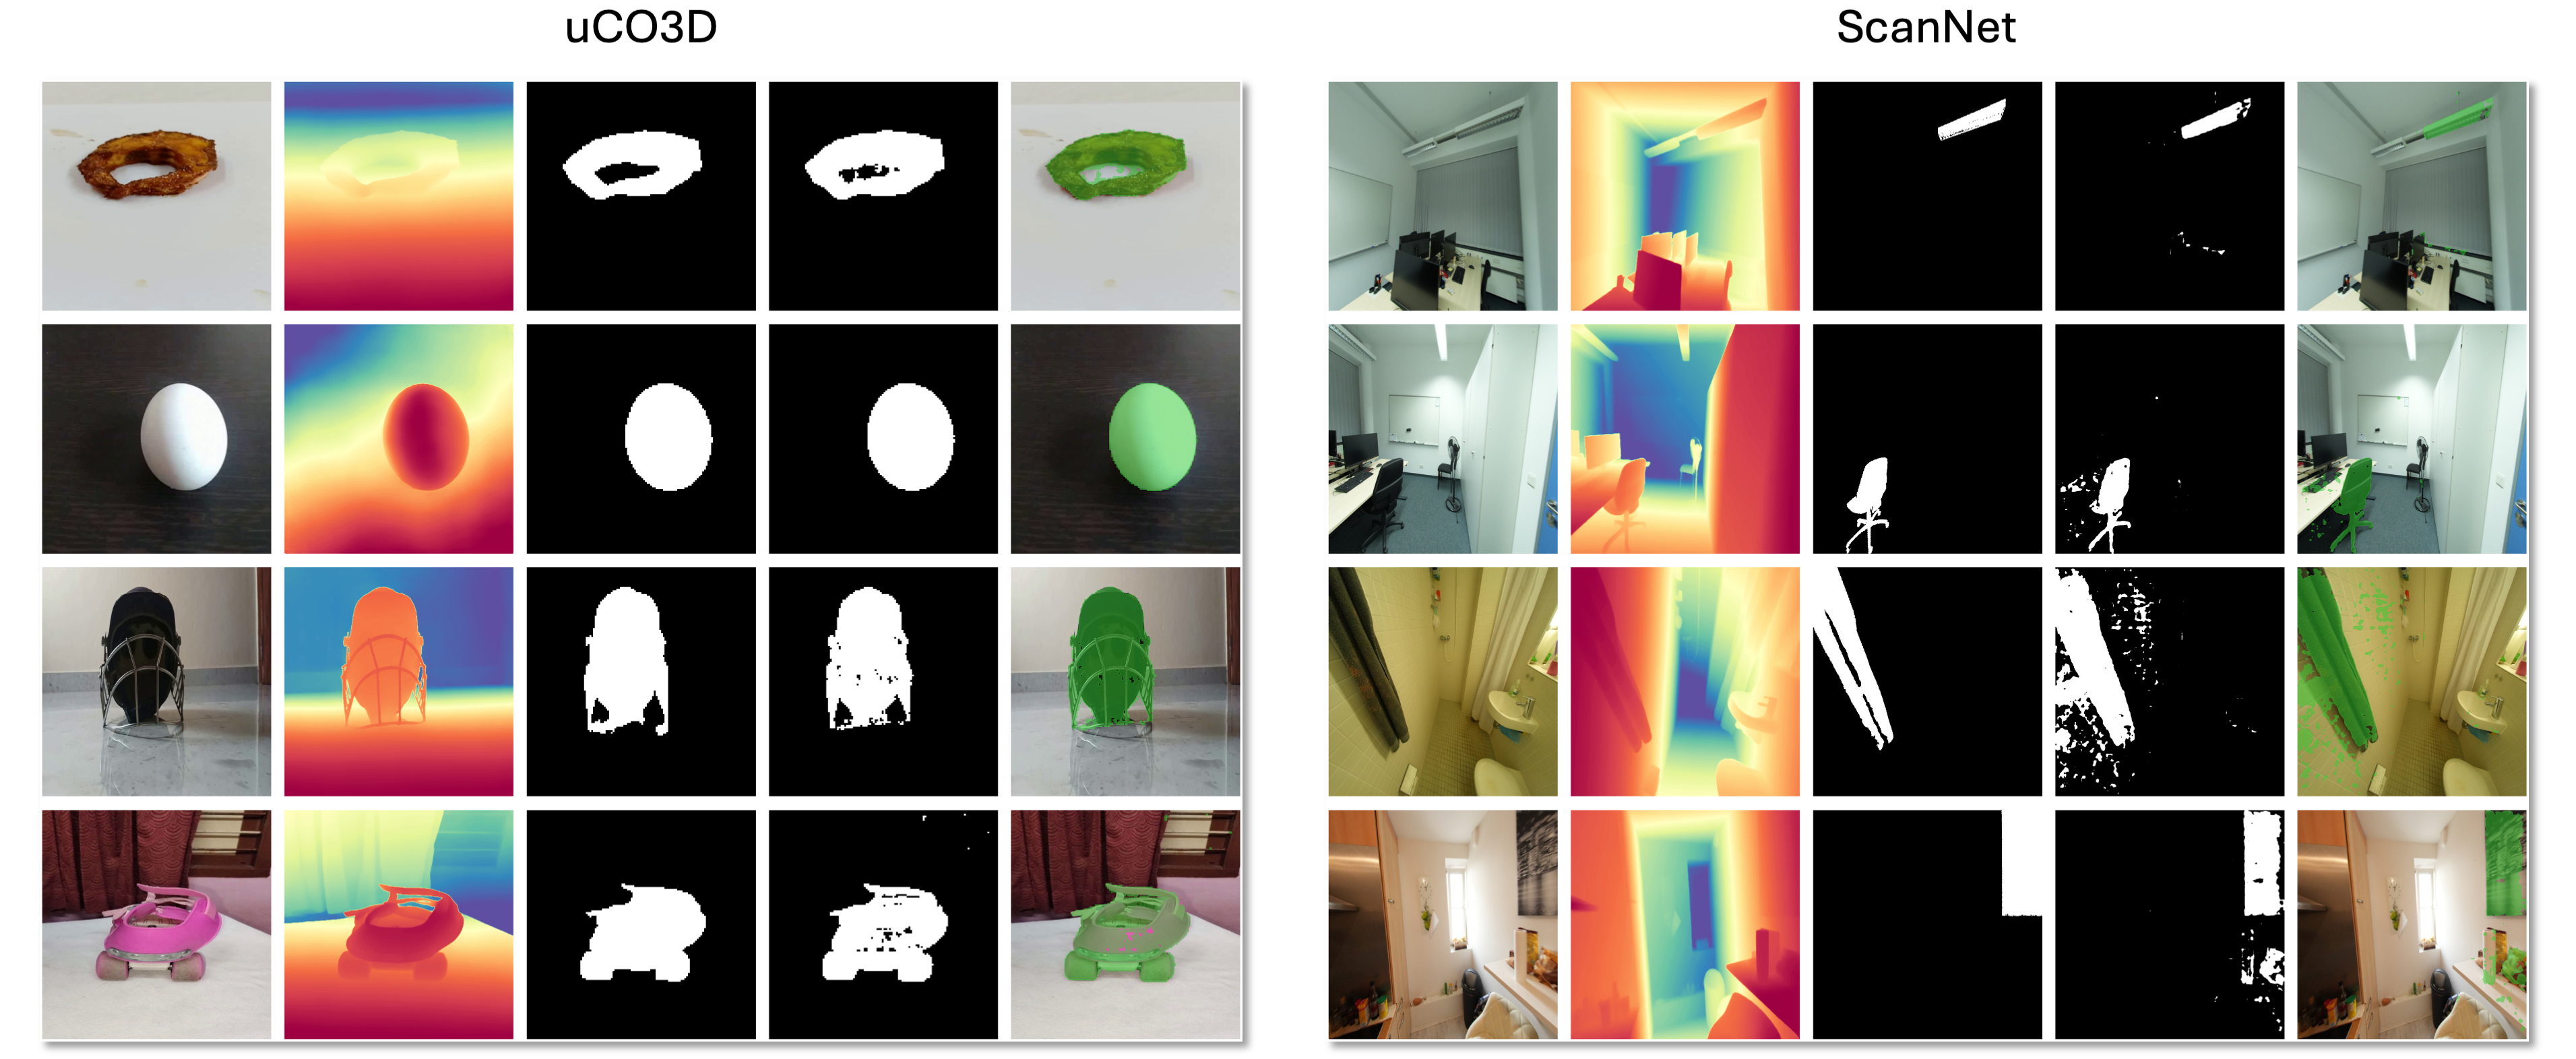
\includegraphics[width=\linewidth]
{figures/grids.png}
\end{center}
\caption{Performance on uCO3D and ScanNet++ datasets. Left-to-right: RGB, depth map, Ground Truth, TrianguLang masks}
\label{fig:grid_uco3d}
\end{figure}

\paragraph{Protocol.}
Following MV-SAM~\cite{mvsam}, we evaluate on 100 frames per scene with 5 randomly sampled objects (excluding structural classes: wall, floor, ceiling). We report mIoU (mean Intersection-over-Union) and mAcc (mean per-class accuracy), averaged across 5 random seeds for object sampling.
\paragraph{Baselines.}
We compare against click-based methods: MV-SAM~\cite{mvsam} (12 grid-sampled point prompts per object, following their published protocol), SAM2-Video~\cite{sam2}, and SAM3~\cite{sam3}; and per-scene optimization methods on NVOS/SPIn-NeRF: SA3D~\cite{SA3D}, SAGA~\cite{SAGA}, OmniSeg3D~\cite{omniseg3d} (using ground-truth 3D reconstructions and calibrated poses). Note that per-scene optimization methods (LERF~\cite{lerf}, LangSplat~\cite{langsplat}) achieve strong accuracy but require calibrated camera poses and 10 to 45 minutes of per-scene training, placing them in a different efficiency regime.

\paragraph{Training.}
Full-scale models train on 230 ScanNet++ scenes (8 views, 100 epochs) or 8,000 uCO3D scenes on 8$\times$ A100 80GB GPUs with DDP. We use AdamW (lr $= 10^{-4}$, cosine schedule, 2-epoch warmup), batch size 8, AMP with FP16, and confidence-based mask selection via align loss~\cite{align2024} at inference.

\subsection{Main Results}

Table~\ref{tab:main} presents in-domain and cross-evaluation results on ScanNet++ and uCO3D. Despite using a single text query instead of 12 click prompts, TrianguLang outperforms all feed-forward baselines in both in-domain and cross-domain settings.

\begin{table}[t]
\caption{In-domain, cross-dataset, and large-scale evaluation results. MV-SAM numbers from~\cite{mvsam}. TrianguLang uses text-only prompts; MV-SAM uses 12 click prompts per object. SA-1B denotes MV-SAM trained on single-view SA-1B data (millions of images).}
\label{tab:main}
\begin{center}
\resizebox{\columnwidth}{!}{
\begin{tabular}{lllcc}
\toprule
Model & Setting & Train $\rightarrow$ Eval & mIoU ($\uparrow$) & mAcc ($\uparrow$) \\
\midrule
\multirow{6}{*}{MV-SAM}
    & In-domain    & ScanNet++ $\rightarrow$ ScanNet++ & 0.510 & 0.694 \\
    & In-domain    & uCo3D $\rightarrow$ uCo3D       & 0.910 & 0.965 \\
    & Cross-domain & uCo3D $\rightarrow$ ScanNet++ & 0.194 & 0.251 \\
    & Cross-domain & ScanNet++ $\rightarrow$ uCo3D   & 0.322 & 0.517 \\
    & Large-scale  & SA-1B $\rightarrow$ ScanNet++    & 0.489 & 0.635 \\
    & Large-scale  & SA-1B $\rightarrow$ uCo3D        & 0.877 & 0.950 \\
\midrule
\multirow{4}{*}{\textbf{TrianguLang (Ours)}}
    & In-domain    & ScanNet++ $\rightarrow$ ScanNet++ & \textbf{0.624} & \textbf{0.774} \\ % v10_full_scale_ep97_seq_proc2; mean_class_recall used as mAcc
    & In-domain    & uCo3D $\rightarrow$ uCo3D       & \textbf{0.946} & \textbf{0.983} \\
    & Cross-domain & uCo3D $\rightarrow$ ScanNet++ & \textbf{0.279} & \textbf{0.685} \\
    & Cross-domain & ScanNet++ $\rightarrow$ uCo3D   & \textbf{0.757} & \textbf{0.796} \\ % v10_full_scale_ep97_uco3d; mean_class_recall
\bottomrule
\end{tabular}
}
\end{center}
\end{table}

\paragraph{In-domain performance.}
On ScanNet++, TrianguLang achieves 62.4\% mIoU with text-only prompts, surpassing MV-SAM's 51.0\% with 12 clicks by 11.4 points (Table~\ref{tab:main}). On uCO3D, the gap is 3.6 points (94.6\% vs.\ 91.0\%). Notably, TrianguLang trained on only 230 ScanNet++ scenes exceeds even MV-SAM trained on the large-scale SA-1B dataset (millions of images) on ScanNet++ evaluation (62.4\% vs.\ 48.9\%), demonstrating that geometric cross-view reasoning compensates for orders-of-magnitude less training data. On uCO3D, MV-SAM's SA-1B variant (87.7\%) benefits from its massive single-view training corpus, but TrianguLang trained in-domain on uCO3D still surpasses it (94.6\% vs.\ 87.7\%).

\textbf{Disentangling backbone from GASA.} SAM3 alone (no cross-view reasoning) achieves only 48.6\% mIoU, \emph{lower} than MV-SAM's 48.9\% (Table~\ref{tab:benchmark_results} in Appendix). TrianguLang's improvement over SAM3-alone confirms that GASA and world-space PE (not the backbone) drive the gains, as quantified in Table~\ref{tab:ablation}.

\paragraph{Oracle vs.\ predicted IoU.}
For transparency, we report oracle mIoU (selecting the GT-best mask among candidates) alongside predicted mIoU. On ScanNet++ (49 val scenes, 100 frames), SAM3 exhibits a \textbf{30-point} oracle-predicted gap (oracle: 79.9\% vs.\ predicted: 49.8\%), because it generates hundreds of mask candidates per scene and struggles to reliably identify the best one. TrianguLang's gap is only \textbf{1 point} (oracle: 63.4\% vs.\ predicted: 62.4\%), demonstrating that our focused 10-query design virtually eliminates mask selection as a bottleneck. Although SAM3's oracle mIoU (79.9\%) substantially exceeds TrianguLang's (63.4\%), its inability to rank candidates correctly results in actual performance 12.6 points \emph{below} TrianguLang.

\paragraph{Cross-domain generalization.}
Cross-dataset transfer reveals the most significant advantage. TrianguLang trained on ScanNet++ achieves 75.7\% mIoU on uCO3D, more than doubling MV-SAM's 32.2\% (+43.5 points). In the reverse direction (uCO3D$\to$ScanNet++), TrianguLang achieves 27.9\% vs.\ 19.4\% (+8.5 points). The asymmetric transfer suggests that diverse indoor viewpoints and occlusion patterns provide more generalizable geometric priors than single-object captures.

\subsection{Multi-View Benchmarks}

On NVOS and SPIn-NeRF, TrianguLang achieves 93.5\% and 91.4\% mIoU respectively, surpassing MV-SAM (92.1\% / 92.5\%) among feed-forward methods while using text instead of clicks. TrianguLang approaches per-scene optimization methods (SAGA: 92.6\% / 93.7\%, SA3D-GS: 92.7\% / 93.4\%) without any per-scene computation; full per-scene results appear in Appendix~\ref{app:benchmarks}.

Tables~\ref{tab:lerf_comparison} and~\ref{tab:lerf_detailed} compare TrianguLang against per-scene optimization methods that embed language features into 3D scene representations on the LERF-OVS benchmark. These methods require calibrated camera poses, 3D reconstruction, and minutes of per-scene training. TrianguLang operates feed-forward without any per-scene computation, representing a fundamentally different efficiency/accuracy tradeoff.

\begin{table}[t]
\centering
\caption{Comparison with per-scene language grounding methods on the LERF-OVS benchmark. Per-scene methods require calibrated poses and scene reconstruction. TrianguLang operates feed-forward using ScanNet++-trained weights without any training on LERF scenes.}
\label{tab:lerf_comparison}
\small
\begin{tabular}{@{}lcccc@{}}
\toprule
\textbf{Method} & \textbf{mIoU} & \textbf{Loc. Acc.} & \textbf{Per-scene} & \textbf{Time} \\
\midrule
LERF~\cite{lerf} & 37.4 & 73.6 & \ding{51} & $\sim$45 min \\
LangSplat~\cite{langsplat} & 51.4 & \textbf{84.3} & \ding{51} & $\sim$10 min \\
LangSplat-V2~\cite{langsplatv2} & \textbf{59.9} & 84.1 & \ding{51} & $\sim$10 min \\
\midrule
\textbf{TrianguLang}$^\dagger$ & 58.1 & 83.5 & \ding{55} & $\sim$58ms \\
\bottomrule
\end{tabular}
\\[1mm]
{\footnotesize $^\dagger$Zero-shot transfer from ScanNet++ (no LERF training). Best in \textbf{bold}.}
\vspace{-2mm}
\end{table}

Without any training on LERF data, TrianguLang achieves 58.1\% mIoU and 83.5\% localization accuracy on LERF-OVS, closely matching the concurrent LangSplat-V2 (59.9\% mIoU, 84.1\% Loc.\ Acc.) while running three orders of magnitude faster ($\sim$58ms vs.\ 10 to 45 min), factoring in LangSplat-V2's per-scene optimization.

\begin{figure}[t]
\centering
\includegraphics[width=\columnwidth]{figures/benchmarking.png}
\caption{Qualitative comparison on LERF-OVS scenes using uniform clip thresholds. Row 1: ``toaster'' query: LERF and LangSplatV2 produce diffuse activations across the scene while TrianguLang tightly focuses its relevancy map on the target object. Row 3: ``stripes'' query: TrianguLang achieves precise localization despite not training on this dataset, and runs 3 orders of magnitude faster ($\sim$58ms vs.\ 10 to 45 min).}
\label{fig:lerf_comparison}
\end{figure}

\begin{table}[h]
\centering
\caption{Per-scene comparison on LERF-OVS benchmark. TrianguLang uses ScanNet++-trained weights without any LERF training (zero-shot transfer). Per-scene methods require 10 to 45 minutes of optimization per scene.}
\label{tab:lerf_detailed}
\resizebox{\linewidth}{!}{
\begin{tabular}{l|ccccc|ccccc}
\toprule
\multirow{2}{*}{\textbf{Method}} & \multicolumn{5}{c|}{\textbf{Localization Accuracy (\%)}} & \multicolumn{5}{c}{\textbf{Semantic Segmentation (mIoU \%)}} \\
 & Ramen & Teatime & Kitchen & Figurines & Overall & Ramen & Teatime & Kitchen & Figurines & Overall \\ \midrule
Gaussian Grouping~\cite{gaussiangrouping} & 32.4 & 69.5 & 50.0 & 44.6 & 49.1 & 26.4 & 54.0 & 31.3 & 34.6 & 36.6 \\
LEGaussians~\cite{legaussians} & 69.0 & 79.7 & 63.6 & 57.1 & 67.4 & 20.2 & 32.3 & 22.3 & 23.4 & 24.6 \\
LERF~\cite{lerf} & 62.0 & 84.8 & 72.7 & 75.0 & 73.6 & 28.2 & 45.0 & 37.9 & 38.6 & 37.4 \\
GOI~\cite{goi} & 56.3 & 67.8 & 68.2 & 44.6 & 59.2 & 33.7 & 55.8 & 54.5 & 23.9 & 42.0 \\
GAGS~\cite{gags} & 69.0 & 88.1 & \underline{90.9} & 78.6 & 81.7 & 46.8 & 60.3 & 55.8 & 53.6 & 54.1 \\
LangSplat~\cite{langsplat} & 73.2 & 88.1 & \textbf{95.5} & \underline{80.4} & \textbf{84.3} & 51.2 & \underline{65.1} & 44.5 & 44.7 & 51.4 \\
\midrule
LangSplat-V2~\cite{langsplatv2} & \underline{74.7} & \textbf{93.2} & 86.4 & 82.1 & \underline{84.1} & \underline{51.8} & \textbf{72.2} & \textbf{59.1} & \underline{56.4} & \textbf{59.9} \\
\midrule
\textbf{TrianguLang}$^\dagger$ & \textbf{75.0} & \underline{88.3} & 83.9 & \textbf{96.6} & 83.5 & \textbf{63.7} & 53.6 & \underline{58.6} & \textbf{56.6} & \underline{58.1} \\
\bottomrule
\end{tabular}}
\\[1mm]
{\footnotesize $^\dagger$Zero-shot transfer from ScanNet++ (no LERF training). Best in \textbf{bold}, second-best \underline{underlined}.}
\end{table}

\subsection{Ablation Studies}

We ablate key components using 230 training scenes with 8 views per scene and sequential sampling, evaluating with matched sampling on 50 held-out scenes (100 frames). Table~\ref{tab:ablation} reports mIoU with changes measured against the full baseline.

\begin{table}[t]
\centering
\caption{Component ablation on ScanNet++ (230 scenes, 8 views, 504 resolution). $\Delta$ measured against ablation baseline (54.7\% mIoU). The full model in Table~\ref{tab:main} achieves 62.4\% at 1008 resolution with 230 scenes.}
\label{tab:ablation}
\small
\begin{tabular}{@{}lcc@{}}
\toprule
\textbf{Configuration} & \textbf{mIoU} & \textbf{$\Delta$} \\
\midrule
Baseline (GASA + World PE) & \textbf{54.7} & $-$ \\
\quad $-$ GASA kernel (standard attn) & 49.4 & $-$5.3 \\
\quad $-$ World-space PE & 49.3 & $-$5.4 \\
\quad $-$ Both (no GASA, no PE) & 46.3 & $-$8.4 \\
\quad RBF kernel (vs.\ learned MLP) & 44.0 & $-$10.7 \\
\bottomrule
\end{tabular}
\vspace{-2mm}
\end{table}

\paragraph{Component contributions.}
Removing the GASA kernel ($-$5.3\%) eliminates the geometric distance bias that suppresses spurious cross-token attention. Without world-space PE ($-$5.4\%), the decoder cannot reason about 3D positions. Removing both components ($-$8.4\%) confirms they are individually critical yet partially complementary: the combined drop is less than the sum of individual drops ($10.7\%$), suggesting shared geometric information.

\subsection{Efficiency}
TrianguLang processes each frame at 1008$\times$1008 resolution in $\sim$58ms on a single A100 GPU, achieving $\sim$17 FPS. With cached depth, preprocessing adds $\sim$32ms per frame ($\sim$90ms total, $\sim$11 FPS). The GASA decoder adds only 13.7M trainable parameters (0.54\% of the 2.54B total), with SAM3 (848M) and DA3-NESTED (1.4B) remaining frozen. For comparison, per-scene optimization methods (SA3D, SAGA, OmniSeg3D) require 30 to 60 minutes of training per new scene; MV-SAM requires 5.1s preprocessing plus 1.1s inference with click prompts. TrianguLang eliminates both per-scene optimization and manual click annotation.


\subsection{Limitations}

\textbf{Depth as bottleneck:} DA3's depth estimates fail on reflective surfaces (mirrors, glass), causing GASA to incorrectly suppress valid correspondences. \textbf{Limited views:} Objects visible in $<$3 views degrade to per-view quality. \textbf{Inherited limitations:} The model inherits SAM3's text-image alignment limitations for rare categories and DA3's metric accuracy ($\sim$5cm error) bounds 3D localization precision. \textbf{Pose estimation on turntable sequences:} DA3-NESTED's pose estimation becomes ill-conditioned on turntable-style captures (e.g., uCO3D) where near-circular camera paths with small baselines cause scale/translation estimation to degenerate; we therefore report only mIoU for uCO3D without Procrustes-aligned 3D localization metrics (ScanNet++ Procrustes alignment remains valid at $\sim$3.9cm median error). \textbf{Training data scale:} TrianguLang was trained on only 230 ScanNet++ scenes, yet outperforms models trained on SA-1B (millions of images); scaling to larger and more diverse training sets would likely amplify the advantage (see Section~\ref{sec:conclusion}).
